\chapter{RESEARCH METHODS}

\begin{figure}[htbp]
	\centering 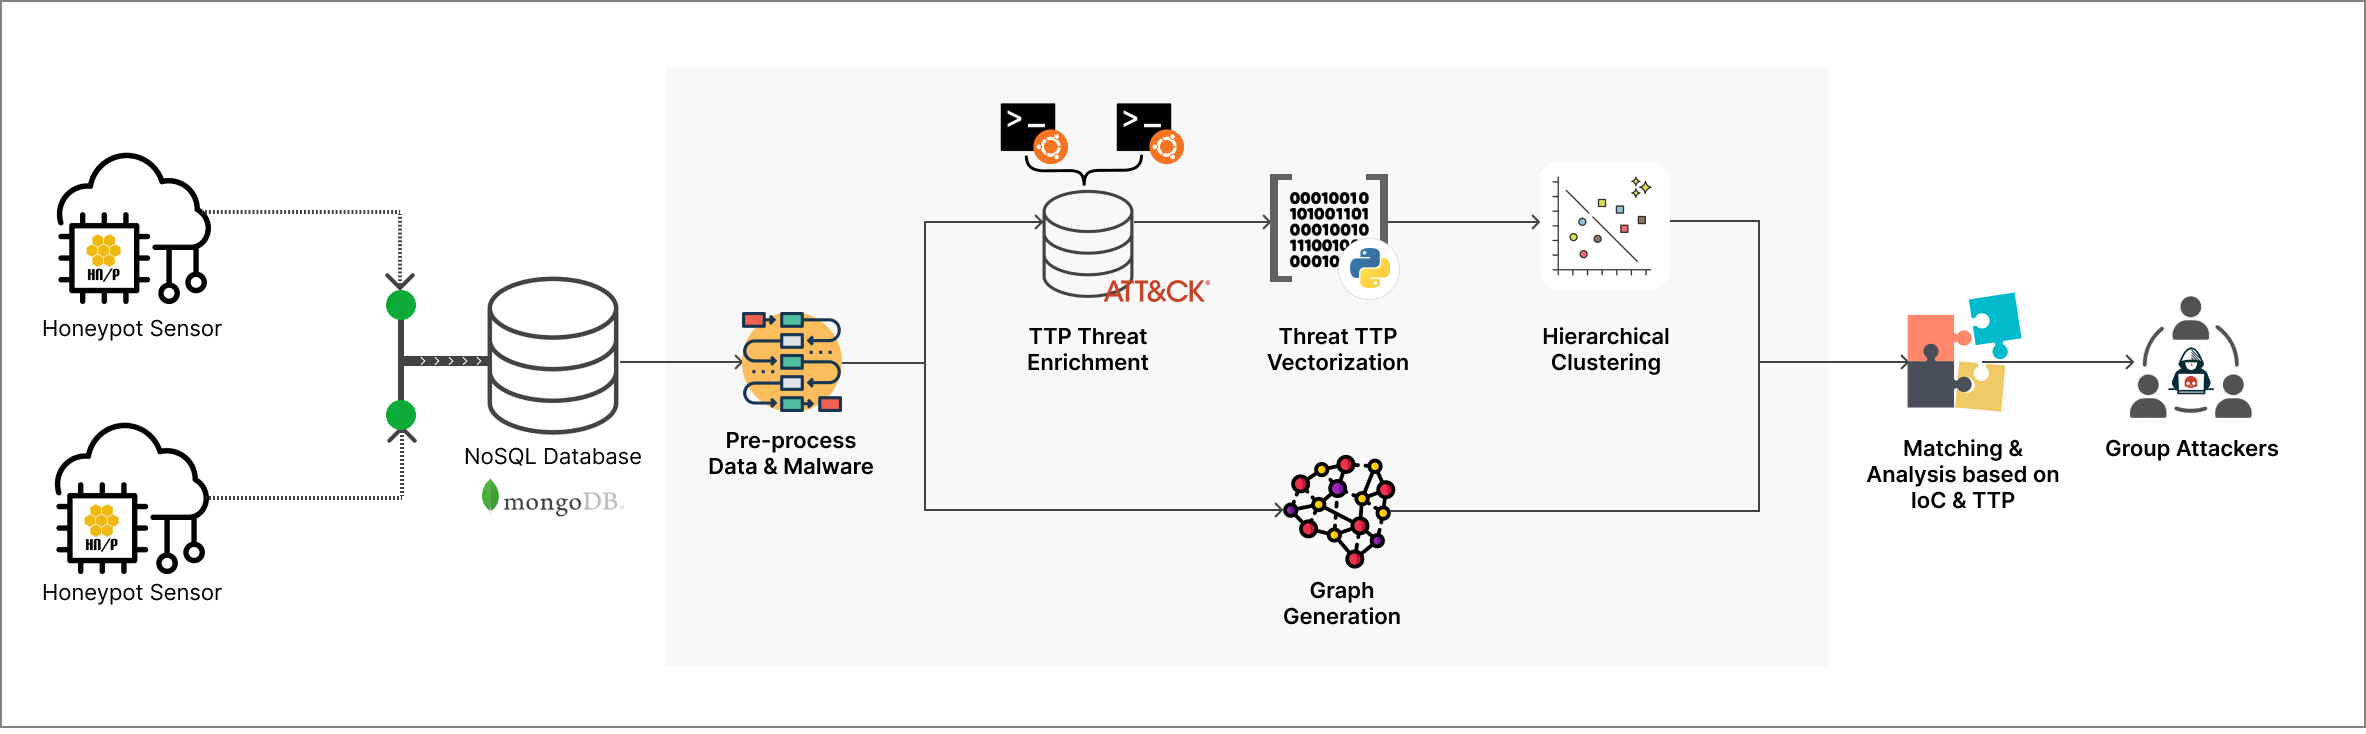
\includegraphics[width=1.0\textwidth]{images/framework.png}
	\caption{Research Framework}
	\label{fig:framework}
\end{figure} 

\section{Research Methodology}
The research methodology section of a thesis is pivotal in ensuring the credibility, validity, and replicability of the study. It serves as the blueprint for conducting the research, like doing literature review, and do some qualitative and/or quantitative methods, detailing how data will be gathered, sample selection, data analysis techniques, and strategies for addressing potential biases. Figure \ref{fig:framework} show the research framework of this research

\section{Research Framework}
A well-crafted research framework serves as the foundational blueprint for any scholarly investigation, providing a clear and structured pathway for the research process. It is essential to begin with a concise and focused thesis statement that articulates the research problem and its significance. Subsequently, the framework should delineate the research objectives, defining what the study aims to achieve. A thorough literature review should be integrated to establish the theoretical and empirical context, identifying gaps and opportunities for contribution. Methodological choices and data collection techniques must be explicitly outlined, ensuring the study's validity and reliability. It’s important the proposed framework includes how to evaluate and validate the research results. A well-structured research framework not only guides the researcher but also enhances the rigor and credibility of the study, ultimately contributing to the advancement of knowledge in the chosen field. Example using STRIDE for Threat Modelling, using NIST SP 800-37 Rev. 2 for Risk Management Framework and many more. 